\documentclass{article}
\usepackage{geometry}
\usepackage{flafter}
\geometry{letterpaper, portrait, margin=1in}

\usepackage{hyperref}
\hypersetup{
    colorlinks=true,
    linkcolor=black,
    filecolor=magenta,
    urlcolor=blue,
}

\usepackage{graphicx}
\graphicspath{ {images/} }

\usepackage{tcolorbox}
\usepackage{textcomp}
\usepackage{gensymb}
\usepackage{indentfirst}

\newcommand{\ans}{$\rule{1.5cm}{0.15mm}$}

\title{RoboJackets Electrical Training Week 0 Worksheet - Answer Key}
\author{Alex Xu}

\begin{document}
\maketitle{}
\setcounter{tocdepth}{2}
\tableofcontents

%Add Preface here

\pagebreak

\section{Intro to Electricity}
\begin{enumerate}
	\item Measured in Ohms ($\ohm$)
	\item $-3.3V-(-5V)=1.7V$
	\item Series, Parallel. Ammeter needs to be in series otherwise it will be shorted. Voltmeters essentially have infinite resistance and if placed in series will make the circuit an open circuit.
	\item $R=V/I=5V/0.2A=25\ohm$
	\item $P=V\dot I = 5V \times 0.2 A = 1W$
	\item $470\ohm \pm 5\%$
\end{enumerate}

\section{Capacitors and Inductors}
\begin{enumerate}
	\item Measured in Faraday ($F$)
	\item $C=Q/V=0.0025C/5V=0.0005F$
	\item False. Electrolytic capacitors have electrolytes inside and have polarity.
	\item False. Electrolytic capacitors are easier to achieve a higher capacitance than ceramics.
	\item Mitigating fluctuation in power supply.
	\item Henry ($H$)
	\item True. For example in solenoids.
	\item False. Inductors are wires wrapped around a coil and display no special characteristics with DC.
\end{enumerate}

\section{Diodes and FETs}
\begin{enumerate}
	\item $5V/20mA=250\ohm$
	\item True. Lots of motors run at 12V and 24V and draws a lot of current while usual logic circuits runs at 5V and below with minimal current involved. Using FETs enables a logic circuit to use minimal power to control the flow of larger power.
	\item Q equals Vss. When A equals Vdd. The upper pFET opens and the lower nFET closes, connecting the output to ground.
\end{enumerate}

\section{Circuit Analysis}
\subsection{Parallel and Series}
	\begin{enumerate}
		\item $R=1/(1/(1.2+1.2)+1/3.6)=1.44$
		\item $ECHO\_OUT=91/(91+47)\times ECHO\_5V\approx 3.297$
		\item $\Sigma C=(10+20+22+100)=152$
		\item $\Sigma C=1/(1/10+1/20+1/22+1/100)\approx 4.8672$
	\end{enumerate}
\subsection{Kirchoff's Law}
	\begin{enumerate}
		\item Let $i_1$ be the current going clockwise in the left loop, $i_2$ be the current through, $R_2$ from top to down and $i_3$ be the current going anti-clockwise in the right loop, then: \par
		$12V = 4\ohm \times i_1 + 3\ohm \times i_2$\par
		$8V = 2\ohm \times i_3 + 3\ohm \times i_2 $\par
		$i_1+i_3=i_2$\par
		solve for $i_1$, $i_2$ and $i_3$, get $i_3 \approx 2.15A$
	\end{enumerate}
	
	\begin{figure}[!h]
		\center
		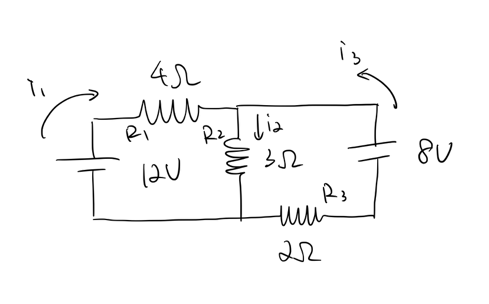
\includegraphics[width=0.4\textwidth, keepaspectratio]{crappyhand}
		\caption{Annotated Circuit}
		\label{fig:kirchoff_hand}
	\end{figure}

\section{Prototyping}
\begin{enumerate}
	\item Not connected, Connected, Not connected
	\item Single core wire, should not. Twisting the wire essentially made the wire into single-core and made metal crimps harder to grab onto the wire.
	\item To eliminate high impedance.
	\item False
\end{enumerate}
\end{document}